\documentclass[12pt,a4paper]{article}
\usepackage[UTF8]{ctex}
\usepackage{geometry}
\usepackage{graphicx}
\usepackage{float}
\usepackage{amsmath}
\usepackage{amsfonts}
\usepackage{amssymb}
\usepackage{booktabs}
\usepackage{multirow}
\usepackage{array}
\usepackage{longtable}
\usepackage{enumerate}
\usepackage{enumitem}  % 添加enumitem包支持自定义列表
\usepackage{fancyhdr}
\usepackage{lastpage}
\usepackage{hyperref}
\usepackage{subcaption}  % 添加子图支持

% 页面设置
\geometry{left=2.5cm,right=2.5cm,top=2.5cm,bottom=2.5cm}

% 行距设置
\linespread{1.2}

% 段落缩进
\setlength{\parindent}{2em}

% 修复页眉高度问题
\setlength{\headheight}{14.49998pt}
\addtolength{\topmargin}{-2.49998pt}

% 页眉页脚设置
\pagestyle{fancy}
\fancyhf{}
\fancyhead[C]{实\hspace{0.5em}验\hspace{0.5em}报\hspace{0.5em}告}
\fancyfoot[C]{\thepage}

\begin{document}

% 正文第一行标题
\noindent
{\Large \textbf{实验八：}\underline{\textbf{元件特性的示波器测量法}}} \hfill {\Large \textbf{实验成绩：}\underline{\hspace{3cm}}}
\vspace{0.5cm}

\section*{一、实验目的}
\begin{enumerate}
    \item 掌握用示波器测量电压、电流等基本量的方法。
    \item 学习用示波器测量信号相位差的方法。
    \item 掌握用示波器测量元件特性的方法。
\end{enumerate}

\section*{二、实验原理}

\subsection*{1. 电压的测量}
示波器测量电压的方法主要有直接测量法和标尺换算法等。在实验中常用直接测量法——从示波器屏幕上直接量出被测电压的高度，换算得电压值。

$$U_{pp} = D_v \cdot h$$

式中，$h$是被测电压信号峰峰值高度(格数)，$D_v$是$Y$轴灵敏度(V/格)。

\textbf{注意：}
\begin{itemize}
    \item 当测量对象是交流电压时，输入耦合方式应选择"AC"；测量直流时选择"DC"。
    \item 测量输入信号之前，先把扫描基线调到合适的参考电平位置。
\end{itemize}

\subsection*{2. 电流的测量}
示波器不能直接测量电流。一般是在该支路中串入一个"采样电阻"$r$，测量该电阻两端的电压$u_r$，由欧姆定律得到电流：

$$i = \frac{u_r}{r}$$

\subsection*{3. 相位差的测量}
测量两个信号的相位差可以用直接法和李萨如图形法等方法。

\begin{itemize}
    \item \textbf{直接法：}把两个信号分别从CH1和CH2输入示波器，开启双踪扫描显示在屏幕上，读出周期格数$T$和相位差格数$\Delta t$，则相位差为：
    $$\varphi = \frac{360^\circ}{T} \cdot \Delta t$$
    
    \item \textbf{李萨如图形法（椭圆法）：}将两个信号分别从CH1和CH2输入示波器，把示波器设置为X-Y显示方式，屏幕上显示椭圆，测量椭圆参数计算相位差：
    $$\varphi = \arcsin\frac{A}{B}$$
    其中$A$为椭圆与$Y$轴的截距，$B$为椭圆的纵轴半径。
\end{itemize}

\subsection*{4. 二端元件特性测量}

\subsubsection*{4.1 电阻元件特性测量}
\begin{itemize}
    \item 示波器选择X-Y显示方式，从CH1输入电阻元件两端的电压信号，从CH2输入电阻元件中流过的电流信号（通过采样电阻$r$测得）。
    \item 采样电阻$r$应满足$R \gg r$的条件，以减少对被测电路的影响。
    \item 屏幕上显示的是电阻的伏安特性曲线，为一条直线。
\end{itemize}

\subsubsection*{4.2 电容元件特性测量}
从CH1和CH2两个通道分别输入电容两端的电压信号和电容电流信号。

根据电容的电压电流关系：
$$u_c = \frac{1}{C} \int i_c(t)dt$$

在正弦激励下，电容电压滞后电流90°，示波器X-Y方式下显示椭圆特性曲线。

\subsubsection*{4.3 电感元件特性测量}
电感元件的特性可以用磁通链-电流（$\psi$-$i$）曲线描述。示波器的CH1和CH2分别输入电流信号和磁通链信号：
$$\psi(t) = \int_0^t u_L(t')dt'$$

其中$u_L$为电感两端电压。

\section*{三、思考题}
\begin{enumerate}
    \item 如何用示波器测量电流？采样电阻$r$的作用是什么？
    
    \textbf{解：}示波器不能直接测量电流，需要通过间接方法测量。具体方法是在待测电流回路中串入一个阻值已知的小电阻$r$（采样电阻），用示波器测量该电阻两端的电压$u_r$，根据欧姆定律计算电流：$i = \frac{u_r}{r}$。
    
    采样电阻的作用是将电流信号转换为电压信号，使示波器能够间接测量电流。采样电阻应满足$R \gg r$的条件，以减少对原电路的影响，避免改变电路的工作状态，保证测量的准确性。
    
    \vspace{1cm}
    
    \item 示波器测量元件特性曲线的原理是什么？为什么必须把显示方式设置成X-Y模式？
    
    \textbf{解：}示波器测量元件特性曲线的原理是：将元件两端的电压信号输入示波器的CH1（X轴），将流过元件的电流信号（通过采样电阻转换的电压信号）输入CH2（Y轴），示波器屏幕上显示的轨迹就是该元件的伏安特性曲线。
    
    必须使用X-Y模式的原因：
    \begin{itemize}
        \item 在X-Y模式下，X轴表示电压，Y轴表示电流，直接显示电压与电流的对应关系，即伏安特性。
        \item 如果使用常规的Y-T模式，X轴表示时间，只能分别观察电压和电流随时间的变化，无法直观地显示电压与电流之间的关系。
        \item X-Y模式能够实时显示元件的静态和动态特性曲线，不同元件呈现不同形状：电阻为直线，电容和电感为椭圆。
    \end{itemize}
    
    \vspace{1cm}
    
    
    
\end{enumerate}

\section*{四、实验任务与线路}
\begin{enumerate}
    \item 用直接法和椭圆图形法测量RC电路的相位差（即$u_c$和$u_s$的相位差），并测量$u_c$的幅值。已知$u_s = 5\sin(800\pi t)$ (V)，写出$u_c$的表达式（其中$R = 510\Omega$，$C = 1\mu F$）
    
    \begin{itemize}
        \item 直接法：画出$u_c$、$u_s$波形，记录数据。
        \item 椭圆图形法：画出X-Y坐标下测量的波形。
    \end{itemize}
    
    \item 测量$R = 510\Omega$电阻元件的伏安特性曲线，$u_s(t) = 5\sin(800\pi t)$ (V)，采样电阻$r = 20\Omega$。
    
    \item 测量非线性电阻元件的端口特性曲线，画出实验线路图。（建议电源$U_{spp} $约为$ 16V$左右）
\end{enumerate}
\begin{figure}[H]
    \centering
    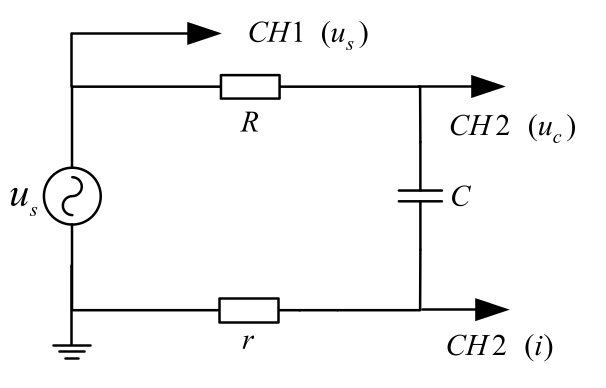
\includegraphics[width=0.8\textwidth]{templete_preview/1.png}
    \caption{实验线路图}
    \label{fig:circuit}
\end{figure}

\begin{figure}[H]
    \centering
    \begin{subfigure}[b]{0.48\textwidth}
        \centering
        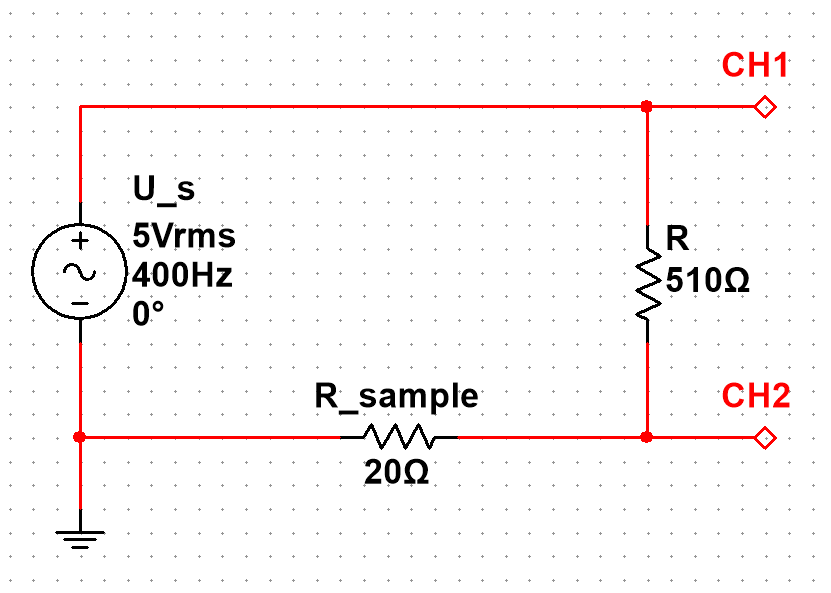
\includegraphics[width=\textwidth]{E8/1.png}
        \caption{$R = 510 \Omega$电阻元件伏安特性测量电路图}
        \label{fig:measure1}
    \end{subfigure}
    \hfill
    \begin{subfigure}[b]{0.48\textwidth}
        \centering
        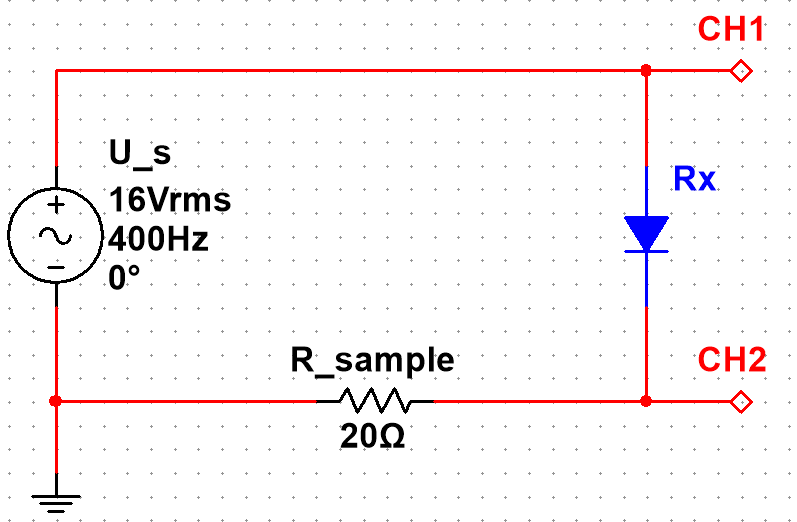
\includegraphics[width=\textwidth]{E8/2.png}
        \caption{非线性电阻元件伏安特性测量电路图}
        \label{fig:measure2}
    \end{subfigure}
    \caption{测量电阻和非线性电阻元件特性电路图}
    \label{fig:resistor_circuits}
\end{figure}

\section*{五、实验数据记录与分析}
\subsection*{1. RC电路相位差测量}
\begin{figure}[H]
    \centering
    \begin{subfigure}[b]{0.64\textwidth}
        \centering
        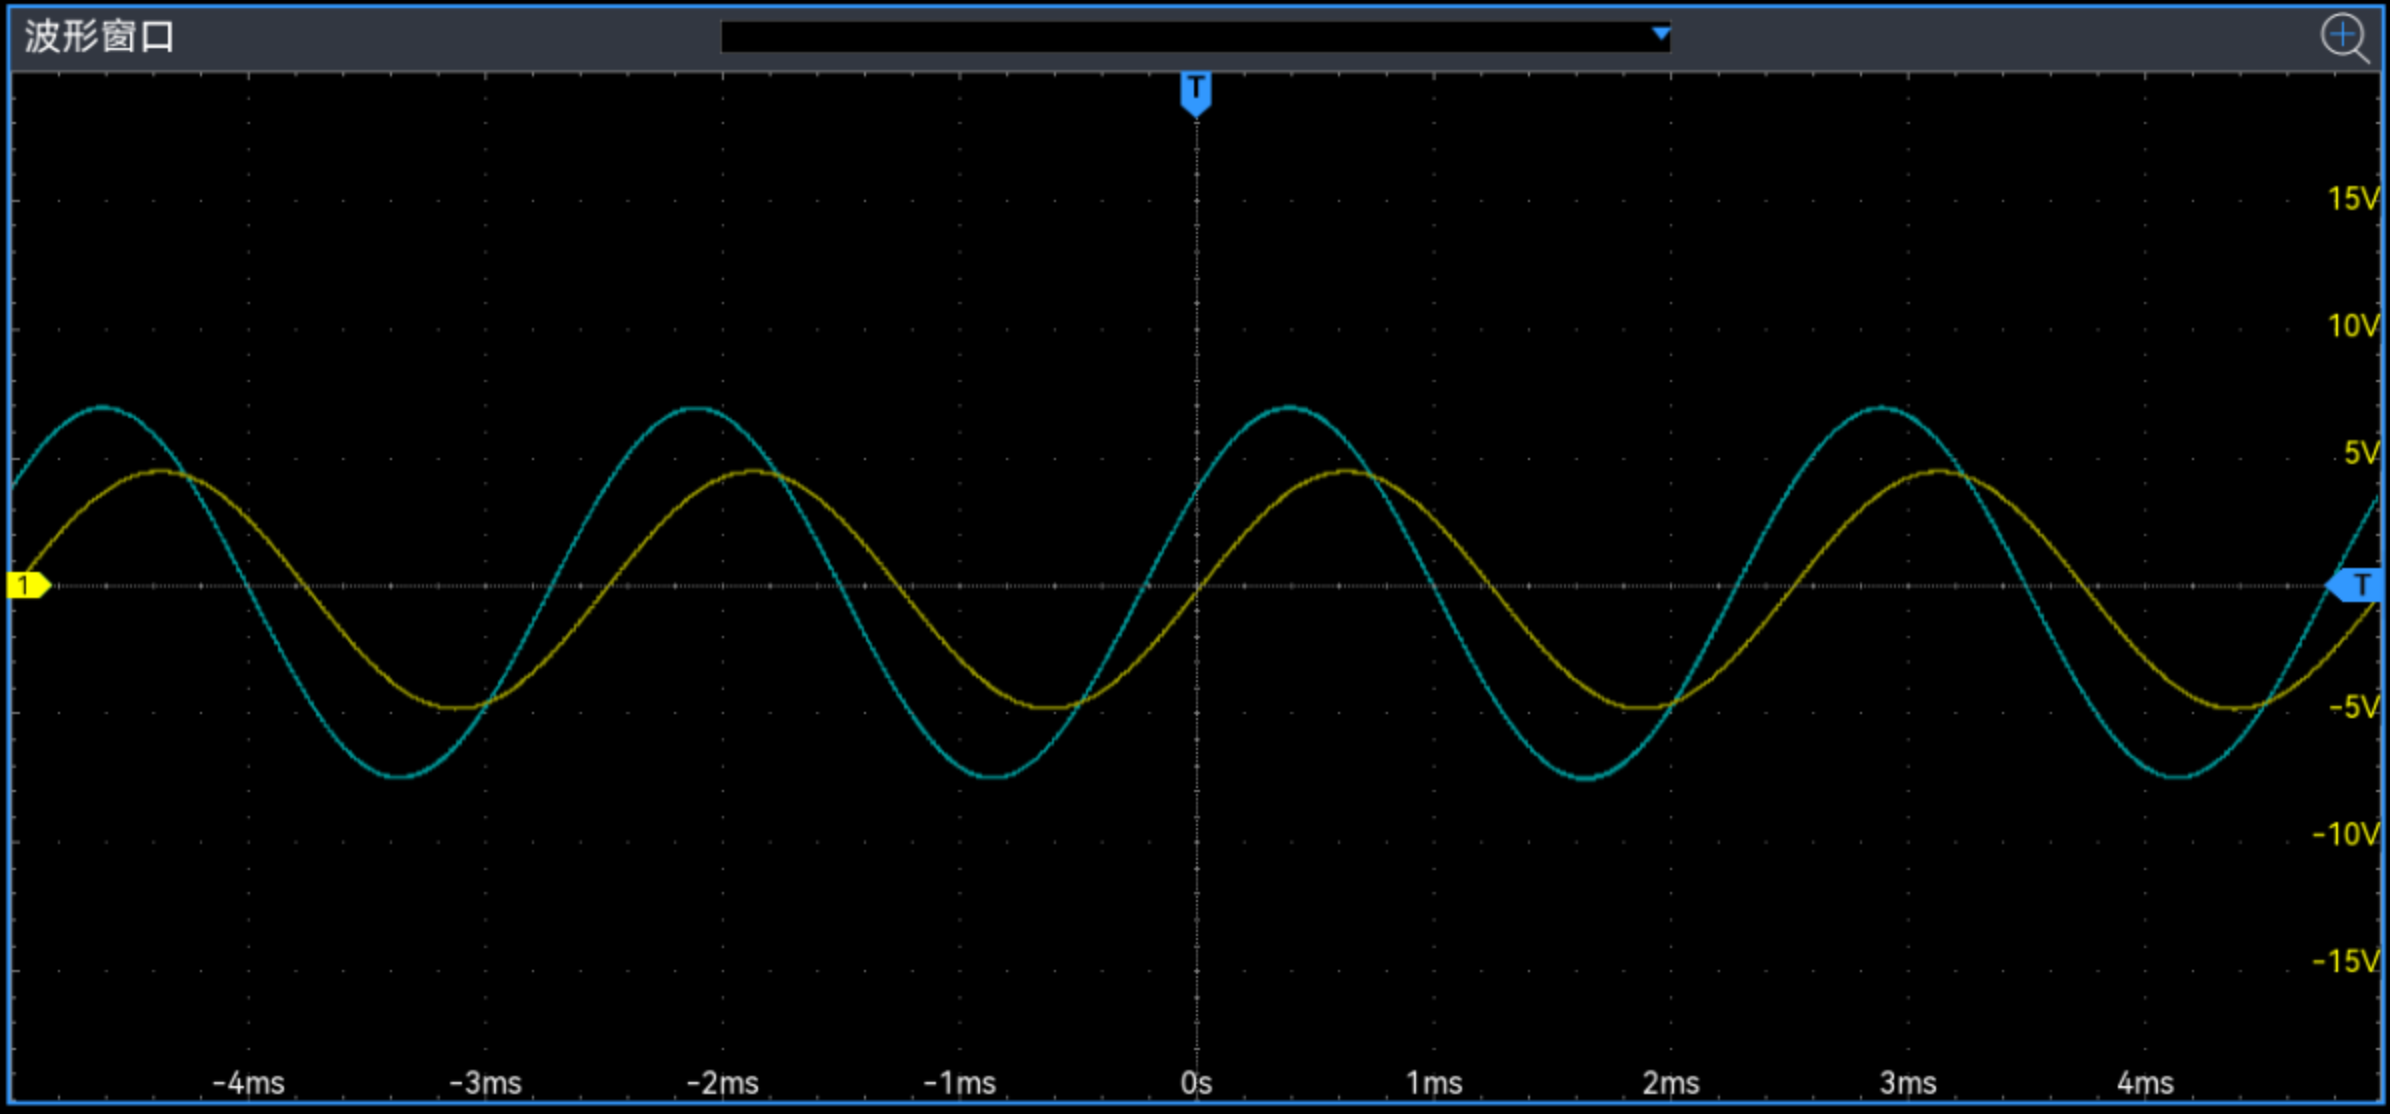
\includegraphics[width=\textwidth]{E8/E1yt.png}
        \caption{直接法测量波形}
        \label{fig:direct_method}
    \end{subfigure}
    \hfill
    \begin{subfigure}[b]{0.32\textwidth}
        \centering
        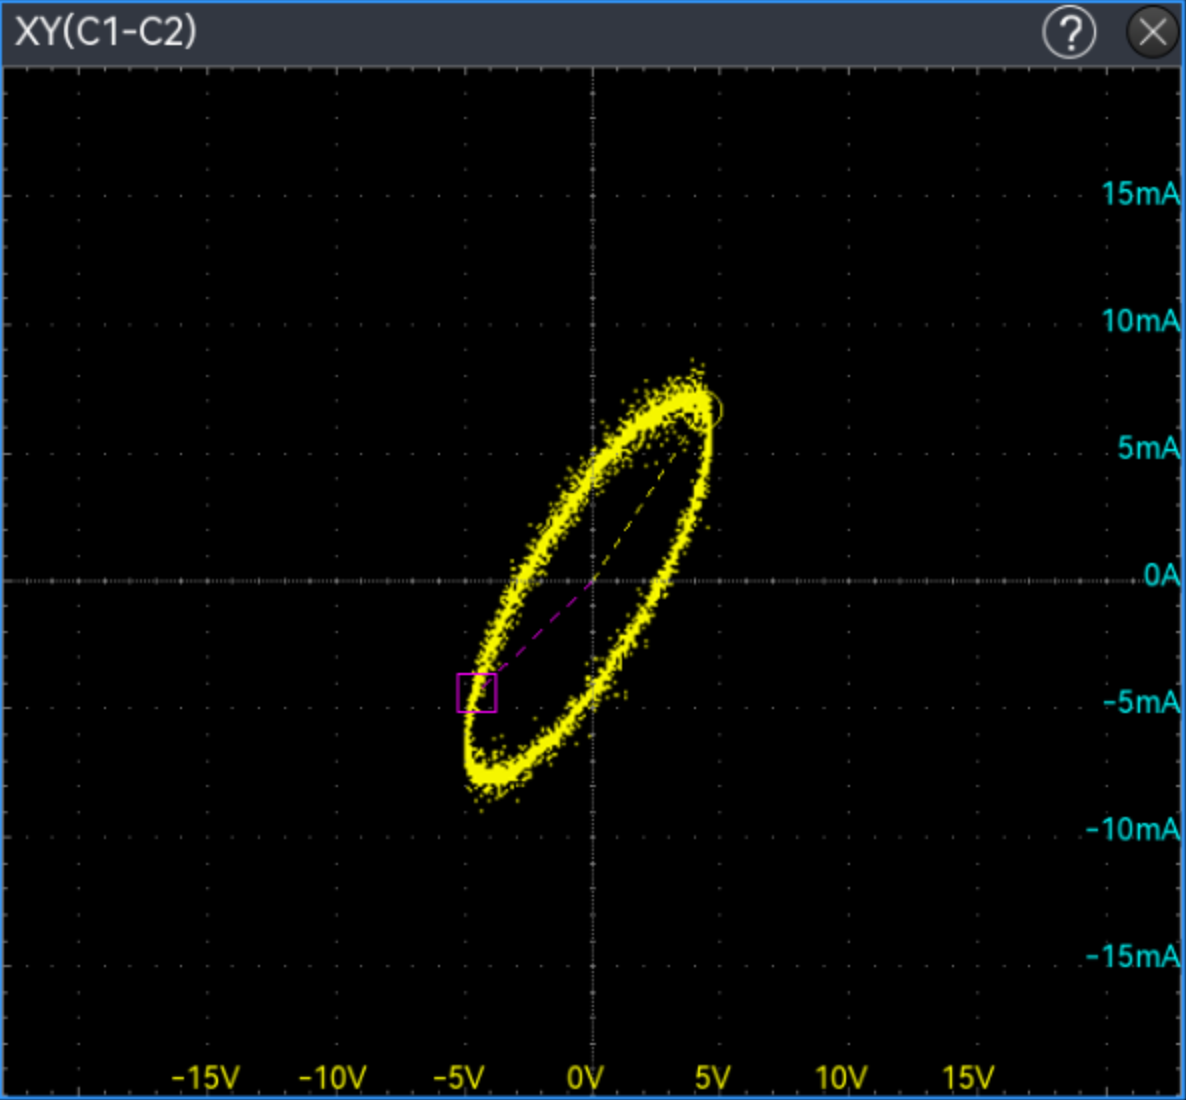
\includegraphics[width=\textwidth]{E8/E1xy.png}
        \caption{椭圆图形法测量}
        \label{fig:ellipse_method}
    \end{subfigure}
    \caption{RC电路相位差测量结果}
    \label{fig:phase_diff}
\end{figure}

\textbf{数据记录：}
\begin{itemize}
    \item 直接法测量数据：$L1 = 376\mu s$，$L2 = 2.48ms$
    \item 椭圆图测量数据：$a = 1.9 V$，$b = 2.368V$
\end{itemize}

\textbf{数据分析：}
\begin{itemize}[label={}]
    \item 直接法测量相位差：
    $$\varphi_1 = \frac{360^\circ}{T} \cdot \Delta t = \frac{360^\circ}{2.48ms} \cdot 376\mu s \approx 54.52^\circ$$
    \item 椭圆图形法测量相位差：
    $$\varphi_2 = \arcsin\frac{A}{B} = \arcsin\frac{1.9V}{2.368V} \approx 53.02^\circ$$
    \item 相对误差：
    $$U_r(\varphi) = \frac{|\varphi_1 - \varphi_2|}{\varphi_2} \times 100\% \approx 2.83\%$$

    误差极小，可认为两种方法测量结果一致。
\end{itemize}

\subsection*{2.$R = 510 \Omega$电阻元件伏安特性测量电路图}

\begin{figure}[H]
    \centering
    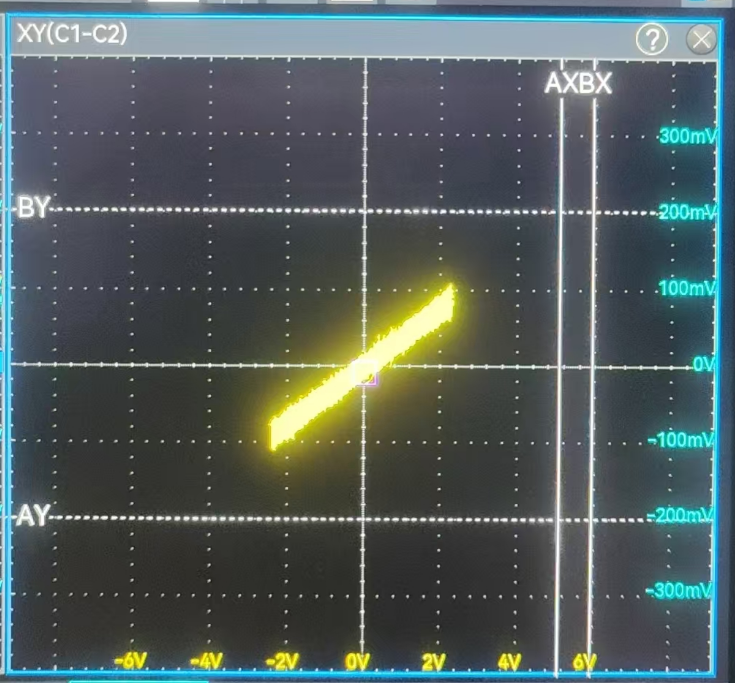
\includegraphics[width=0.6\textwidth]{E8/E2.png}
    \caption{电阻元件伏安特性曲线}
    \label{fig:resistor_va}
\end{figure}

\textbf{数据记录：}
\begin{itemize}
    \item $U_{CH1} = 4.5010V$， $U_{CH2} = 172.91mV$， $r = 20\Omega$， $R = 510\Omega$
\end{itemize}

\textbf{数据分析：}
\begin{itemize}[label={}]
    \item 回路中电流：
    $$I = \frac{U_{CH2}}{r} = \frac{172.91mV}{20\Omega} \approx 8.6455mA$$
    \item 回路总电阻：
    $$R_{total} = \frac{U_{CH1}}{I} = \frac{4.5010V}{8.6455mA} \approx 520.6\Omega$$
    \item 被测电阻：
    $$R_{measure} = R_{total} - r \approx 500.6\Omega$$
    \item 相对误差：
    $$U_r(R) = \frac{|R_{measure} - R|}{R} \times 100\% \approx 1.84\%$$
    \item 误差较小，测量结果较为准确。
\end{itemize}

\subsection*{3. 非线性电阻元件伏安特性测量电路图}

\begin{figure}[H]
    \centering
    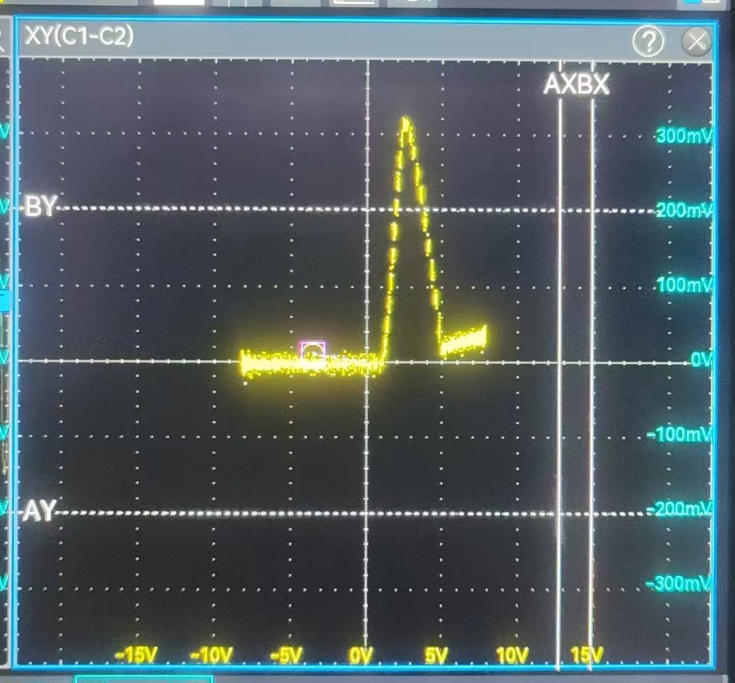
\includegraphics[width=0.6\textwidth]{E8/E3.png}
    \caption{非线性电阻元件伏安特性曲线}
    \label{fig:nonlinear_resistor_va}
\end{figure}

\textbf{数据分析：}
\begin{itemize}[label={}]
    \item 非线性电阻元件的伏安特性曲线如图所示，斜率不断变化，呈现出非线性关系，符合预期。
\end{itemize}

\subsection*{4.总阻抗的测量}
\begin{figure}[H]
    \centering
    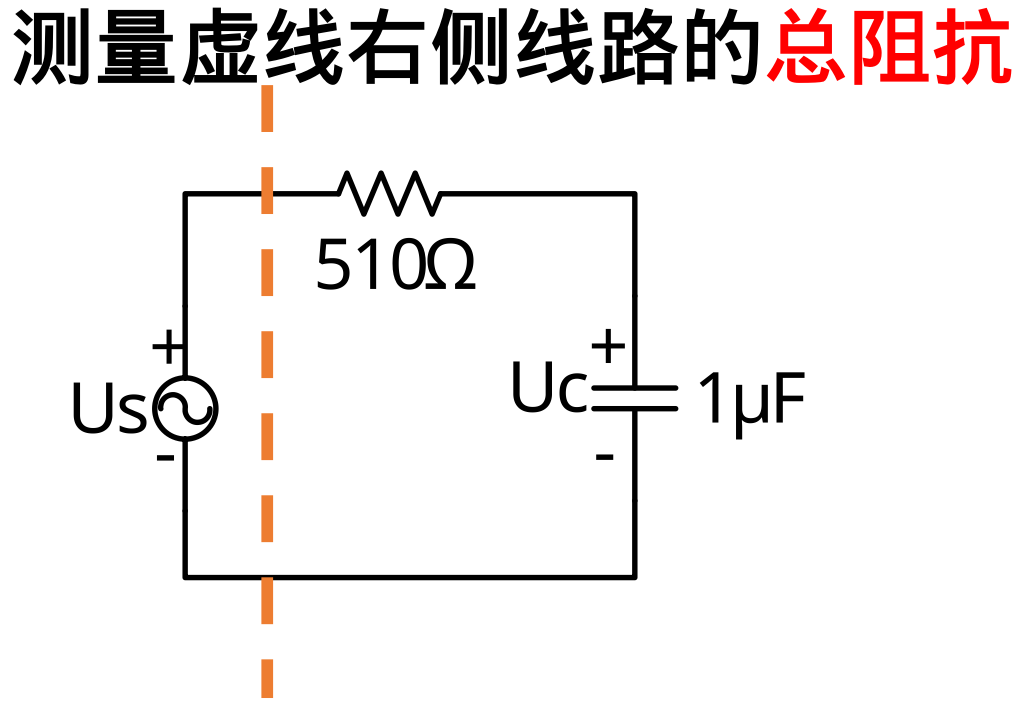
\includegraphics[width=0.6\textwidth]{E8/image.png}
    \caption{测量虚线右侧电路的总阻抗}
    \label{fig:nonlinear_resistor_va1}
\end{figure}

\textbf{数据记录：}
\begin{itemize}
    \item $U_{CH1} = 9.200V$， $I_{CH2} = 14.400mA$， $r = 20\Omega$， $R = 510\Omega$，$C = 1\mu F$，$f = 400Hz$
\end{itemize}





\textbf{数据分析：}
\begin{itemize}[label={}]
    \item 总阻抗理论值:
     $$|Z_{theoretical}| = \sqrt{R^2 + ({\frac{1}{j \omega C}})^2} =\sqrt{{530\Omega}^2+ ({\frac{1}{j \times 2\pi \times 400Hz \times 1\mu F}})^2  } =  662.73\Omega$$
    \item 总阻抗实际值：
    $$|Z_{measured}| = \frac{U_{CH1}}{I_{CH2}} =\frac{9.200V}{14.400mA} = 638.89\Omega$$ 
    \item 相对误差：
    $$U_r(|Z|) = \frac{||Z_{measure}| - |Z_{theoretical}||}{||Z_{theoretical}||} \times 100\% \approx 3.60\%$$
\end{itemize}



\section*{六、实验小结}
通过本次实验，我学会了用示波器测量电压、电流等基本电学量，并掌握了用直接法和李萨如图形法测量相位差的方法。同时通过搭建包含电阻、电容、电感元件的电路，成功测量出各元件的特性曲线。

实验中，我深入理解了X-Y显示模式在元件特性测量中的重要作用，了解了不同元件特性曲线的形状特点：电阻呈直线特性，电容和电感呈椭圆特性。对于RC移相电路，通过测量不同频率下的相位差和幅值，加深了对电路频率响应的认识。

此次实验让我对示波器的功能及工作原理有了更进一步的了解，提高了使用示波器进行电路分析和测量的实践能力。

\end{document}